
\documentclass[11pt]{article}
\usepackage[a4paper,margin=1in]{geometry}
\usepackage{amsmath,amssymb}
\usepackage{graphicx}
\usepackage[dvipsnames]{xcolor}
\usepackage{hyperref}
\usepackage{enumitem}
\usepackage{tabularx}
\usepackage{longtable}
\usepackage{booktabs}
\usepackage[most]{tcolorbox}
\usepackage{titlesec}
\usepackage{xurl}
\usepackage{fancyhdr}
\usepackage{setspace}
\usepackage{tikz}
\usetikzlibrary{positioning,arrows.meta}
\usepackage[T1]{fontenc}
\usepackage{lmodern}
\setlength{\parindent}{0pt}
\setlength{\parskip}{8pt}
\setlength{\headheight}{14pt}
\setstretch{1.12}
\setlist[itemize]{leftmargin=1.5em, nosep}
\setlist[enumerate]{leftmargin=1.5em, nosep}
\providecommand{\tightlist}{\setlength{\itemsep}{0pt}\setlength{\parskip}{0pt}}
\hypersetup{colorlinks=true,linkcolor=MidnightBlue,urlcolor=MidnightBlue}
\pagestyle{fancy}
\fancyhf{}
\rhead{\thepage}
\renewcommand{\headrulewidth}{0pt}
\renewcommand{\footrulewidth}{0pt}
\titleformat{\section}{\Large\bfseries\color{MidnightBlue}}{\thesection}{0.6em}{}
\titleformat{\subsection}{\bfseries}{}{0em}{}


\begin{document}

\begin{center}\LARGE\bfseries Modern Coding Agents and KG Reasoning\end{center}

\begin{center}\large Block 3 Day 5\end{center}

\begin{tcolorbox}[colback=MidnightBlue!4,colframe=MidnightBlue,title={Session Overview},fonttitle=\bfseries,breakable]
\textbf{Session objective:} Evaluate coding-agent workflows, risk controls, and where structured repository knowledge improves software changes.

\textbf{Timing target (min):} 70

\textbf{Topic anchors:} coding agent; planner; tester; reviewer; impact analysis; prompt injection; secret leakage

\textbf{Padlet board:} \url{https://padlet.com/qmul/b3-d5-mjxv8jfjor5277z8}
\end{tcolorbox}

\section*{Exercises}

\begin{tcolorbox}[colback=white,colframe=MidnightBlue,title={Q1 Core Concept Check},fonttitle=\bfseries,breakable]
\begin{center}
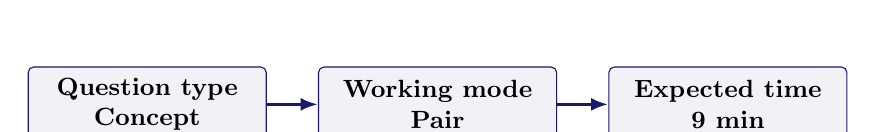
\begin{tikzpicture}[
node distance=0.65cm,
box/.style={draw=MidnightBlue, rounded corners=2pt, minimum height=0.95cm, align=center, font=\small\bfseries, fill=MidnightBlue!6, text width=0.23\linewidth},
arrow/.style={-{Latex[length=2.2mm]}, very thick, MidnightBlue}
]
\node[box] (type) {Question type\\Concept};
\node[box, right=of type] (mode) {Working mode\\Pair};
\node[box, right=of mode] (time) {Expected time\\9 min};
\draw[arrow] (type) -- (mode);
\draw[arrow] (mode) -- (time);
\end{tikzpicture}
\end{center}

{\large\bfseries\color{MidnightBlue} Prompt}\par\medskip
Explain the planner-coder-tester-reviewer workflow of a coding agent in simple language. Then add one sentence on what makes this workflow different from a chatbot that only answers questions.

{\large\bfseries\color{MidnightBlue} Task details}\par\medskip
\begin{itemize}\item \textbf{Type:} concept
\item \textbf{Mode:} pair
\item \textbf{Time:} 9 min
\item \textbf{Deliverable:} workflow summary
\item \textbf{Assessment focus:} explain what makes a coding agent different from a normal chatbot
\item \textbf{Expected length:} 4 role bullets + 1 sentence\end{itemize}

{\large\bfseries\color{MidnightBlue} How to submit}\par\medskip
Post one pair Padlet comment listing the four roles and one short difference statement.

{\large\bfseries\color{MidnightBlue} Discussion in class}\par\medskip
Which role disappears first if the system becomes unsafe and overconfident?

{\large\bfseries\color{MidnightBlue} Why this helps}\par\medskip
Useful for short questions on coding-agent architecture and acting versus chatting.

{\large\bfseries\color{MidnightBlue} References}\par\medskip
\begin{itemize}\item Russell \& Norvig (2021) AIMA 4e, Ch.10, pp.314-343
\item Poole \& Mackworth (2023) 3e, Ch.16-17, pp.701-766
\item https://openai.com/codex/\end{itemize}
\end{tcolorbox}

\begin{tcolorbox}[colback=white,colframe=MidnightBlue,title={Q2 Structured Problem},fonttitle=\bfseries,breakable]
\begin{center}
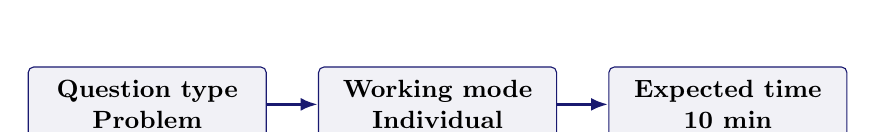
\begin{tikzpicture}[
node distance=0.65cm,
box/.style={draw=MidnightBlue, rounded corners=2pt, minimum height=0.95cm, align=center, font=\small\bfseries, fill=MidnightBlue!6, text width=0.23\linewidth},
arrow/.style={-{Latex[length=2.2mm]}, very thick, MidnightBlue}
]
\node[box] (type) {Question type\\Problem};
\node[box, right=of type] (mode) {Working mode\\Individual};
\node[box, right=of mode] (time) {Expected time\\10 min};
\draw[arrow] (type) -- (mode);
\draw[arrow] (mode) -- (time);
\end{tikzpicture}
\end{center}

{\large\bfseries\color{MidnightBlue} Prompt}\par\medskip
A coding agent has been asked to fix a payment bug. Before it edits any code, what context should it gather? List six items drawn from the lecture, such as task goal, relevant files, tests, policies, dependencies, or likely impact area.

{\large\bfseries\color{MidnightBlue} Task details}\par\medskip
\begin{itemize}\item \textbf{Type:} problem
\item \textbf{Mode:} individual
\item \textbf{Time:} 10 min
\item \textbf{Deliverable:} context checklist
\item \textbf{Assessment focus:} identify the minimum repository context a coding agent should gather before editing
\item \textbf{Expected length:} 6 items\end{itemize}

{\large\bfseries\color{MidnightBlue} How to submit}\par\medskip
Post your own Padlet comment as a six-item checklist.

{\large\bfseries\color{MidnightBlue} Discussion in class}\par\medskip
Which missing context item is most likely to cause a wrong edit?

{\large\bfseries\color{MidnightBlue} Why this helps}\par\medskip
Direct practice for questions on context collection and responsible agent action.

{\large\bfseries\color{MidnightBlue} References}\par\medskip
\begin{itemize}\item Russell \& Norvig (2021) AIMA 4e, Ch.10, pp.314-343
\item Poole \& Mackworth (2023) 3e, Ch.16-17, pp.701-766
\item https://openai.com/codex/
\item https://docs.anthropic.com/en/docs/claude-code/overview\end{itemize}
\end{tcolorbox}

\begin{tcolorbox}[colback=white,colframe=MidnightBlue,title={Q3 Structured Problem},fonttitle=\bfseries,breakable]
\begin{center}
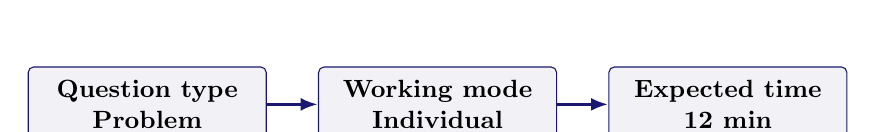
\begin{tikzpicture}[
node distance=0.65cm,
box/.style={draw=MidnightBlue, rounded corners=2pt, minimum height=0.95cm, align=center, font=\small\bfseries, fill=MidnightBlue!6, text width=0.23\linewidth},
arrow/.style={-{Latex[length=2.2mm]}, very thick, MidnightBlue}
]
\node[box] (type) {Question type\\Problem};
\node[box, right=of type] (mode) {Working mode\\Individual};
\node[box, right=of mode] (time) {Expected time\\12 min};
\draw[arrow] (type) -- (mode);
\draw[arrow] (mode) -- (time);
\end{tikzpicture}
\end{center}

{\large\bfseries\color{MidnightBlue} Prompt}\par\medskip
For an enterprise payment-service repository, score these four risks from 1-5 on likelihood and impact: prompt injection from repository text, secret leakage, unsafe command execution, and passing tests with the wrong fix. Then say which one you would mitigate first.

{\large\bfseries\color{MidnightBlue} Task details}\par\medskip
\begin{itemize}\item \textbf{Type:} problem
\item \textbf{Mode:} individual
\item \textbf{Time:} 12 min
\item \textbf{Deliverable:} risk table
\item \textbf{Assessment focus:} prioritise repository risks for a coding-agent workflow
\item \textbf{Expected length:} 4 rows\end{itemize}

{\large\bfseries\color{MidnightBlue} How to submit}\par\medskip
Post your own Padlet comment as a four-row table plus one short priority statement.

{\large\bfseries\color{MidnightBlue} Discussion in class}\par\medskip
Which risk looks small at first but can become catastrophic later?

{\large\bfseries\color{MidnightBlue} Why this helps}\par\medskip
Direct practice for safety-risk prioritisation questions involving coding agents.

{\large\bfseries\color{MidnightBlue} References}\par\medskip
\begin{itemize}\item Russell \& Norvig (2021) AIMA 4e, Ch.10, pp.314-343
\item Poole \& Mackworth (2023) 3e, Ch.16-17, pp.701-766
\item https://genai.owasp.org/resource/agentic-ai-threats-and-mitigations/\end{itemize}
\end{tcolorbox}

\begin{tcolorbox}[colback=white,colframe=MidnightBlue,title={Q4 Collaborative Mini-Case},fonttitle=\bfseries,breakable]
\begin{center}
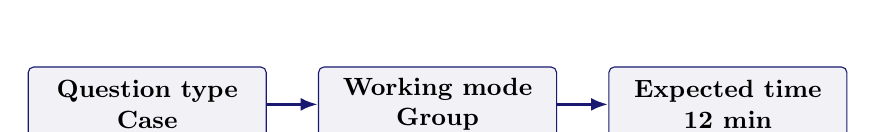
\begin{tikzpicture}[
node distance=0.65cm,
box/.style={draw=MidnightBlue, rounded corners=2pt, minimum height=0.95cm, align=center, font=\small\bfseries, fill=MidnightBlue!6, text width=0.23\linewidth},
arrow/.style={-{Latex[length=2.2mm]}, very thick, MidnightBlue}
]
\node[box] (type) {Question type\\Case};
\node[box, right=of type] (mode) {Working mode\\Group};
\node[box, right=of mode] (time) {Expected time\\12 min};
\draw[arrow] (type) -- (mode);
\draw[arrow] (mode) -- (time);
\end{tikzpicture}
\end{center}

{\large\bfseries\color{MidnightBlue} Prompt}\par\medskip
Design a safe pull-request workflow for a payment bug fix using planner, coder, tester, and reviewer agents. Your workflow must include one repository-memory or impact-analysis step and one human approval gate before merge.

{\large\bfseries\color{MidnightBlue} Task details}\par\medskip
\begin{itemize}\item \textbf{Type:} case
\item \textbf{Mode:} group
\item \textbf{Time:} 12 min
\item \textbf{Deliverable:} PR workflow design
\item \textbf{Assessment focus:} design a safe pull-request workflow with impact analysis and a human gate
\item \textbf{Expected length:} 6 steps\end{itemize}

{\large\bfseries\color{MidnightBlue} How to submit}\par\medskip
Post one group Padlet comment with the role order, the memory or impact-analysis step, and the human gate.

{\large\bfseries\color{MidnightBlue} Discussion in class}\par\medskip
Where should the human reviewer intervene if only one checkpoint is allowed?

{\large\bfseries\color{MidnightBlue} Why this helps}\par\medskip
Supports case questions on safe orchestration of coding agents inside real software workflows.

{\large\bfseries\color{MidnightBlue} References}\par\medskip
\begin{itemize}\item Russell \& Norvig (2021) AIMA 4e, Ch.10, pp.314-343
\item Poole \& Mackworth (2023) 3e, Ch.16-17, pp.701-766
\item https://openai.com/codex/
\item https://docs.replit.com/replitai/agent\end{itemize}
\end{tcolorbox}

\begin{tcolorbox}[colback=white,colframe=MidnightBlue,title={Q5 Exam-Style Constructed Response},fonttitle=\bfseries,breakable]
\begin{center}
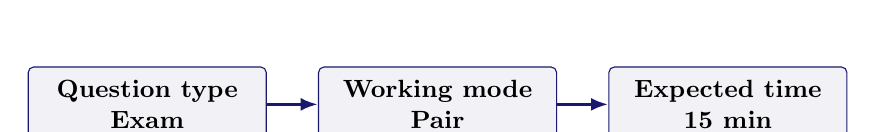
\begin{tikzpicture}[
node distance=0.65cm,
box/.style={draw=MidnightBlue, rounded corners=2pt, minimum height=0.95cm, align=center, font=\small\bfseries, fill=MidnightBlue!6, text width=0.23\linewidth},
arrow/.style={-{Latex[length=2.2mm]}, very thick, MidnightBlue}
]
\node[box] (type) {Question type\\Exam};
\node[box, right=of type] (mode) {Working mode\\Pair};
\node[box, right=of mode] (time) {Expected time\\15 min};
\draw[arrow] (type) -- (mode);
\draw[arrow] (mode) -- (time);
\end{tikzpicture}
\end{center}

{\large\bfseries\color{MidnightBlue} Prompt}\par\medskip
Argue for a minimum safe operating standard for coding agents in production repositories. Your answer must include approval, tool limits, and audit trail.

{\large\bfseries\color{MidnightBlue} Task details}\par\medskip
\begin{itemize}\item \textbf{Type:} exam
\item \textbf{Mode:} pair
\item \textbf{Time:} 15 min
\item \textbf{Deliverable:} justified essay
\item \textbf{Assessment focus:} argue for a minimum safe operating standard for coding agents
\item \textbf{Expected length:} 180-240 words\end{itemize}

{\large\bfseries\color{MidnightBlue} How to submit}\par\medskip
Post one pair Padlet comment with a clear standard, the reasons behind it, and one example of what it prevents.

{\large\bfseries\color{MidnightBlue} Discussion in class}\par\medskip
Which safety rule would product teams be most tempted to remove?

{\large\bfseries\color{MidnightBlue} Why this helps}\par\medskip
Matches long-form exam questions on governance, trust, and operational safeguards for coding agents.

{\large\bfseries\color{MidnightBlue} References}\par\medskip
\begin{itemize}\item Russell \& Norvig (2021) AIMA 4e, Ch.10, pp.314-343
\item Poole \& Mackworth (2023) 3e, Ch.16-17, pp.701-766
\item https://genai.owasp.org/resource/agentic-ai-threats-and-mitigations/\end{itemize}
\end{tcolorbox}

\begin{tcolorbox}[colback=white,colframe=MidnightBlue,title={Q6 Stretch Extension},fonttitle=\bfseries,breakable]
\begin{center}
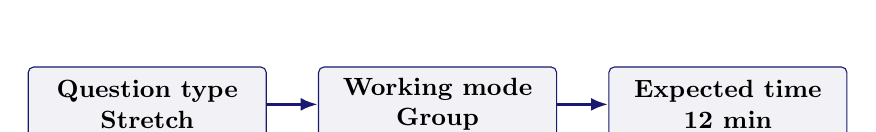
\begin{tikzpicture}[
node distance=0.65cm,
box/.style={draw=MidnightBlue, rounded corners=2pt, minimum height=0.95cm, align=center, font=\small\bfseries, fill=MidnightBlue!6, text width=0.23\linewidth},
arrow/.style={-{Latex[length=2.2mm]}, very thick, MidnightBlue}
]
\node[box] (type) {Question type\\Stretch};
\node[box, right=of type] (mode) {Working mode\\Group};
\node[box, right=of mode] (time) {Expected time\\12 min};
\draw[arrow] (type) -- (mode);
\draw[arrow] (mode) -- (time);
\end{tikzpicture}
\end{center}

{\large\bfseries\color{MidnightBlue} Prompt}\par\medskip
Build a tiny repository graph for a payment bug fix. Include at least five nodes such as service, endpoint, database table, test suite, and policy file, then draw or describe the links and explain how this graph would help impact analysis.

{\large\bfseries\color{MidnightBlue} Task details}\par\medskip
\begin{itemize}\item \textbf{Type:} stretch
\item \textbf{Mode:} group
\item \textbf{Time:} 12 min
\item \textbf{Deliverable:} tiny repository graph
\item \textbf{Assessment focus:} show where structured repository knowledge helps impact analysis
\item \textbf{Expected length:} 5 nodes + 4 links + 1 explanation\end{itemize}

{\large\bfseries\color{MidnightBlue} How to submit}\par\medskip
Post one group Padlet comment with the nodes, the links, and one short explanation of how the graph reduces risk.

{\large\bfseries\color{MidnightBlue} Discussion in class}\par\medskip
Which edge in your repository graph would be easiest to miss but most dangerous to ignore?

{\large\bfseries\color{MidnightBlue} Why this helps}\par\medskip
Good extension for synthesis questions on why structured repository knowledge helps coding agents.

{\large\bfseries\color{MidnightBlue} References}\par\medskip
\begin{itemize}\item Russell \& Norvig (2021) AIMA 4e, Ch.10, pp.314-343
\item Poole \& Mackworth (2023) 3e, Ch.16-17, pp.701-766
\item https://qwenlm.github.io/qwen-code-docs/en/users/overview/
\item https://docs.z.ai/guides/llm/glm-5.1\end{itemize}
\end{tcolorbox}

\section*{Submission Instructions}

Use the seeded Padlet posts for Q1--Q6. Q2 and Q3 are individual. Q1 and Q5 are pair tasks. Q4 and Q6 should be one joint group comment. Start each comment with your names or group label.

\section*{Whole-Class Debrief Prompts}

\begin{itemize}
\tightlist
\item
  What context should a coding agent never skip before editing code?
\item
  Which risk deserves the earliest hard guardrail?
\item
  Where does a small repository graph help more than a flat file list?
\end{itemize}

\section*{Exam Transfer Note (Day-Level)}

Maps to exam questions on coding-agent workflow, context collection, risk assessment, safe PR orchestration, governance, and graph-supported impact analysis.

\end{document}
